\chapter{Progettazione e codifica}
\label{cap:progettazione-codifica}

\lstset{
    escapeinside={(*@}{@*)}, % Delimitatori per modalità LaTeX
    basicstyle=\ttfamily,    % Stile monospaziato
}

\intro{Questo capitolo è incentrato sulla progettazione e sulla codifica dell'algoritmo, mostrando passo per passo il suo funzionamento}


\section{Progettazione}

Questa sezione esplora i diversi aspetti fondamentali nella progettazione di un algoritmo genetico: le componenti fondamentali, la struttura e gli operatori genetici.

\subsection{Composizione degli algoritmi evolutivi}

I principali componenti di ricerca per progettare un algoritmo evolutivo sono i seguenti:

\begin{itemize}
    \item \textbf{Rappresentazione}: negli algoritmi genetici, la soluzione codificata è chiamata cromosoma, mentre le variabili decisionali all'interno di una soluzione (cromosoma) sono i geni;
    
    \item \textbf{Inizializzazione della popolazione}: la generazione della popolazione iniziale è un aspetto cruciale in quanto una giusta inizializzazione determina un vantaggio già dalle prime interazioni;
    
    \item \textbf{Funzione di fitness}: si tratta della funzione obbiettivo, ogni soluzione ha un valore di fitness che indica il grado di adeguatezza rispetto al problema;
    
    \item \textbf{Strategia di selezione}: la strategia di selezione affronta la seguente domanda: "Quali genitori per la prossima generazione vengono scelti con un bias verso un fitness migliore?";
    
    \item \textbf{Strategia di riproduzione}: la strategia di riproduzione consiste nel progettare operatori di mutazione e crossover adeguati per generare nuovi individui (discendenti);
    
    \item \textbf{Strategia di sostituzione}: i nuovi discendenti competono con gli individui più vecchi per ottenere il loro posto nella prossima generazione (sopravvivenza del più adatto);
    
    \item \textbf{Criteri di arresto}: determina la fine del loop evolutivo, solitamente è indicato come il numero di generazioni da raggiungere, ovvero ogni interazione è una generazione.
\end{itemize}

\subsection{Struttura del genetico}

In questa sezione descriviamo la struttura dell'Algoritmo Genetico scelta per il controllo delle sue fasi di intensificazione e diversificazione.
L'obiettivo è massimizzare una funzione di fitness $f$. I parametri richiesti dall'algoritmo GA sono:

\begin{itemize}
    \item $N$: dimensione della popolazione;
    \item $p_c$: probabilità di crossover;
    \item $p_m$: probabilità di mutazione;
    \item $M$: dimensione del pool di accoppiamento;
    \item $E$: dimensione dell'élite.
\end{itemize}

Indichiamo con $P$ la popolazione di cromosomi e con $G$ l'insieme di discendenti generati dalla fase di riproduzione.

\begin{lstlisting}
def GA(N, pc, pm, M, E):
    P = generate(N);
    while not terminate() do
        G = reproduction(P, pc, pm, M);
        P = replace(P, G, E);
    end
    return maxf P;
end
\end{lstlisting}

\subsubsection{Riproduzione}
In questa fase utilizziamo operatori binari (crossover) e unari (mutazione) per esplorare altre soluzioni alterando solo una parte della soluzione. Questa modifica parziale (invece di una riorganizzazione totale, che sarebbe una ricerca casuale), insieme al sostegno degli individui più idonei (es. selezione dei genitori), porta l'algoritmo a spingere avanti nelle generazioni le soluzioni più idonee mantenendo un buon tasso di esplorazione di nuovi cromosomi. La dimensione dei discendenti richiesta è pari alla dimensione della popolazione $N$, che poi subisce la procedura di sostituzione.

La probabilità di riproduzione indicata con $Be(p)$, ovvero, la variabile casuale di Bernoulli che assume valore 1 con probabilità $p$ e 0 con probabilità $1-p$.

\begin{lstlisting}
    def Reproduction(P, pc, pm, M):
        G = [ ];
        pool = sortf(P)[0 : M];
        while not |G| == |P| do
            par1, par2 = selection(pool);
            if Be(pc) == 1 then
                c1, c2 = crossover(par1, par2);
            else
                c1, c2 = par1, par2;
            end
            G = G (*@$\cup$@*) {c1, c2};
        end
        foreach g (*@$\in$@*) G do
            if Be(pm) == 1 then
                mutation(c);
            end
        end
        return G;
    end
\end{lstlisting}

\subsubsection{Rimpiazzo}
La strategia di rimpiazzo ha un grande impatto sull'intensificazione. La metodologia di rimpiazzo adottata può essere spiegata in due passaggi: 
\begin{enumerate}
    \item i migliori $E$ elementi nell'unione di $P$ e $G$ fanno automaticamente parte della popolazione successiva;
    \item i migliori $|P| - E$ discendenti di $G$ sono inclusi nella popolazione successiva.
\end{enumerate}

\begin{lstlisting}
    def Replace(P, G, E):
        elite = best subset(P (*@$\cup$@*) G, E, f);
        Gbest = best subset(G, |P| - E, f);
        return elite (*@$\cup$@*) Gbest;
    end
\end{lstlisting}

\subsection{Operatori genetici}

Gli operatori genetici permettono agli algoritmi evolutivi di modulare la diversificazione. Operano sui cromosomi alterandone i geni e permettendo di esplorare un ampio spazio di soluzioni senza andare a perdere intensificazione grazie alla selezione e all'elitismo.

\subsubsection{Selezione}

La selezione dei genitori viene effettuata sui migliori \( M \) individui della popolazione attuale, i quali costituiscono il cosiddetto \emph{Mating Pool}.

Il meccanismo di selezione è uno dei principali componenti di ricerca negli algoritmi evolutivi (EAs). Il principio fondamentale dei metodi di selezione è: \emph{"più un individuo è valido, maggiore è la sua probabilità di essere scelto come genitore."} Questa pressione selettiva guida la popolazione verso soluzioni migliori. Tuttavia, gli individui peggiori non dovrebbero essere completamente scartati, poiché essi potrebbero contenere materiale genetico utile.

La strategia di selezione determina quali individui vengono scelti per l'accoppiamento (riproduzione).

La selezione tramite ruota della roulette è la strategia di selezione più comune. Essa assegna a ciascun individuo una probabilità di selezione proporzionale alla sua fitness relativa. Sia $f_i$ la fitness dell'individuo $p_i$ nella popolazione $P$. La probabilità di selezione è data da:

\[ p_i = \frac{f_i}{\sum_{j=1}^{n} f_j} \]

Immaginiamo un grafico a torta in cui a ciascun individuo è assegnato uno spazio proporzionale alla sua fitness. Una ruota della roulette è posizionata attorno al grafico. La selezione di $\mu$ individui avviene tramite $\mu$ spin indipendenti della ruota. Ogni spin seleziona un singolo individuo. Gli individui migliori occupano più spazio e, di conseguenza, hanno maggiori probabilità di essere scelti (Figura 5.2).

\begin{figure}[!ht] 
    \centering 
    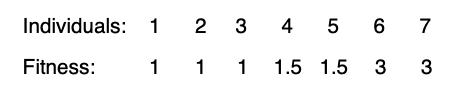
\includegraphics[width=0.6\columnwidth]{tesi/fitness_roulette_wheel} 
    \caption{Pesi della ruota}
\end{figure}

\begin{figure}[!ht] 
    \centering 
    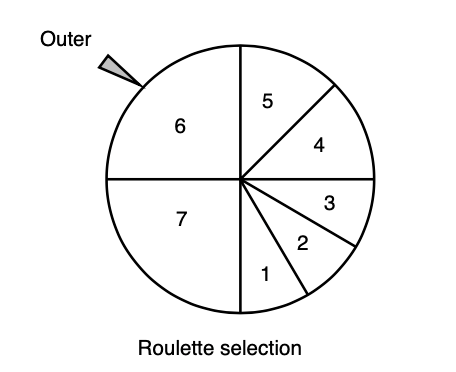
\includegraphics[width=0.6\columnwidth]{tesi/roulette_wheel} 
    \caption{Grafico a torta della selezione tramite ruota della roulette}
\end{figure}

Tuttavia, nella selezione tramite ruota della roulette, individui eccezionali possono introdurre un bias all'inizio della ricerca, causando una convergenza prematura e una perdita di diversità genetica. Infatti, va notato che un valore di \( M \) troppo piccolo intensifica il focus sui migliori individui del \emph{Mating Pool}, riducendo però la diversificazione della popolazione. Questo compromesso deve essere attentamente bilanciato per garantire un efficace equilibrio tra esplorazione e sfruttamento nel processo evolutivo.

\subsubsection{Crossover}
Il crossover prende i due genitori selezionati e genera due figli da aggiungere ai nuovi discendenti. Un crossover avviene con una probabilità $p_c$, altrimenti i genitori vengono semplicemente clonati e aggiunti ai discendenti. L'operatore di crossover, da un lato, mescola i geni delle coppie di cromosomi esplorando nuove soluzioni; dall'altro, se la diversità genetica (individui diversi) nella popolazione è bassa, può portare a una convergenza prematura. Nel caso estremo in cui abbiamo una popolazione composta da elementi tutti uguali, il crossover non può creare nuovi individui. Per garantire la diversità genetica, si può ridurre la fase di intensificazione (es. $E$ o $M$) o aumentare il tasso di mutazione $p_m$.

A differenza degli operatori unari, come la mutazione, l'operatore di crossover è binario e talvolta n-ario. Il ruolo degli operatori di crossover è di ereditare alcune caratteristiche dei due genitori per generare i discendenti. Come per l'operatore di mutazione, la progettazione degli operatori di crossover dipende principalmente dalla rappresentazione utilizzata.

Applicare operatori di crossover classici alle permutazioni, come nel nostro caso, genera soluzioni che non sono permutazioni (ossia, soluzioni non valide). Di conseguenza, sono stati progettati numerosi operatori di crossover per permutazioni, tra cui il crossover a ordine (OX). Per prima cosa, due punti di crossover vengono selezionati casualmente. Dal genitore 1, si copia nel discendente, alle stesse posizioni assolute, la parte tra i due punti. Dal genitore 2, si parte dal secondo punto di crossover e si scelgono gli elementi non già selezionati dal genitore 1, inserendoli nel discendente a partire dal secondo punto di crossover. L'operatore di crossover OX è un operatore di pura ricombinazione. Se si inizia a riempire o scegliere dal primo punto di crossover, l'operatore non sarà puro. Dal genitore 1, vengono preservati l'ordine relativo, l'adiacenza e le posizioni assolute. Dal genitore 2, viene preservato solo l'ordine relativo.

\begin{figure}[!ht] 
    \centering 
    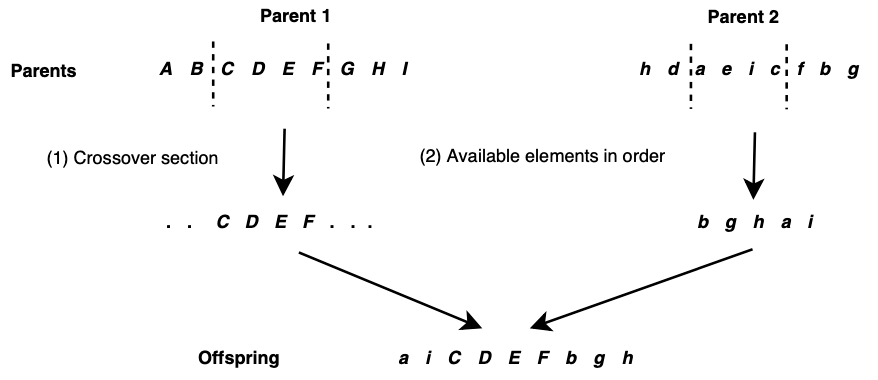
\includegraphics[width=1\columnwidth]{tesi/OXCrossover} 
    \caption{Rappresentazione del crossover OX}
\end{figure}

\subsubsection{Mutazione}
La mutazione viene eseguita dopo il crossover e crea una perturbazione casuale del cromosoma selezionato. Il ruolo della mutazione è duplice: da un lato, simile all'operatore di crossover, provoca una perturbazione di una soluzione per favorire l'esplorazione; dall'altro aumenta la diversità genetica anche se l'attuale diversità è scarsa. Questo è in contrasto con il crossover, che non può diversificare molto un set di individui molto simili.

Gli operatori di mutazione sono operatori unari che agiscono su un singolo individuo. Le mutazioni rappresentano piccoli cambiamenti degli individui selezionati nella popolazione. La probabilità $p_m$ definisce la probabilità di mutare ogni elemento (gene) della rappresentazione. Alcune strategie inizializzano la probabilità di mutazione a $1/k$, dove $k$ è il numero di variabili decisionali, in modo che in media solo poche variabili vengano mutate.

Alcuni punti importanti da considerare nella progettazione o nell'uso di un operatore di mutazione sono i seguenti:

\begin{itemize}
    \item \textbf{Ergodicità}: l'operatore di mutazione dovrebbe consentire di raggiungere ogni soluzione nello spazio di ricerca.
    \item \textbf{Validità}: l'operatore di mutazione dovrebbe produrre soluzioni valide. Questo non è sempre possibile nei problemi di ottimizzazione vincolati.
    \item \textbf{Località}: la mutazione dovrebbe produrre un cambiamento minimo. La dimensione della mutazione è importante e dovrebbe essere controllabile. La località è l'effetto sulla soluzione (fenotipo) quando si esegue la modifica (perturbazione) nella rappresentazione (genotipo). Quando vengono effettuati piccoli cambiamenti nel genotipo, il fenotipo deve rivelare piccoli cambiamenti. In questo caso, si dice che la mutazione ha una forte località. Una debole località è caratterizzata da un grande effetto sul fenotipo quando viene effettuato un piccolo cambiamento nel genotipo.
\end{itemize}

La mutazione in rappresentazioni basate sull'ordine, come nel nostro caso, è generalmente basata sugli operatori di scambio (swapping), inversione o inserimento. 

\section{Parametrizzazione}

In questa sezione viene discussa e motivata la scelta dei valori dei parametri dell'algoritmo tenendo contro delle caratteristiche da ottimizzare, delle istanze di prova fornite dall'azienda e di possibili rischi di overtuning.

L'obbiettivo è quello scegliere una configurazione ottimale di parametri dell'algoritmo per cercare di ottimizzare le seguenti caratteristiche:
\begin{itemize}
	\item\textbf{Intensificazione}: ci si aspetta che il valore di fitness della soluzione migliore all'interno della popolazione incrementi nel corso delle generazioni;
	\item\textbf{Diversificazione}: l'algoritmo deve esplorare un vasto insieme di soluzioni, gli operatori di crossover e mutazione potranno generare soluzioni con valori fitness inferiori a quello della peggiore soluzione della generazione precedente. Quando questo avviene significa che l'algoritmo sta esplorando anche soluzioni diverse, tuttavia non è necessariamente indice che l'esplorazione avvenga in maniera sufficente;
	\item\textbf{Costo computazionale}: come vedremmo in seguito, il criterio di arresto dei test svolti sull'algoritmo è un limite di tempo impostato a 30 secondi. In base all'istanza, è possibile che in 30 secondi vengano computizzate 10 o 100 generazioni. Siccome gli algoritmi genetici sono progettati per funzionare al meglio con l'incrementarsi di generazioni, il limite di tempo non è un criterio di arresto ottimale, tuttavia è necessario per confronti o test. Questo rende la velocità di esecuzione un aspetto di cui tenere conto per permettere all'algoritmo di eseguire più generazioni possibili nel tempo limite.
\end{itemize}

\subsection{Scelta delle configurazioni}

I parametri da configurare sono:
\begin{itemize}
	\item\textbf{population\_size}: dimensione della popolazione di cromosomi, ovvero le soluzioni sul quale lavora il genetico;
	\item\textbf{crossover\_prob}: probabilità che l'algoritmo svolga l'operazione di crossover (applicata a coppie di soluzioni presenti nella pool);
	\item\textbf{mutation\_prob}: probabilità che l'algoritmo svolga l'operazione di mutazione (applicata a ogni soluzione presente nella pool);
	\item\textbf{mating\_pool\_size}: dimensione del pool di accoppiamento;
	\item\textbf{elite\_size}: dimensione dell'insieme dei migliori cromosomi della popolazione che verranno inseriti direttamente nella popolazione della generazione successiva.
\end{itemize}

\noindent La configurazione iniziale (fornita dal tutor aziendale sulla base risultati ottenuti per un algoritmo genetico svolto su un altro problema) è, \textbf{Conf1}:
\begin{itemize}
	\item\textbf{population\_size}: 50;
	\item\textbf{crossover\_prob}: 0,7 (70\%);
	\item\textbf{mutation\_prob}: 0,3 (30\%);
	\item\textbf{mating\_pool\_size}: 20;
	\item\textbf{elite\_size}: 5.
\end{itemize}

Di seguito verranno mostrati alcuni grafici di test svolti su delle singole istanze di prova, fornite appositamente dall'azienda, allo scopo di mostrare l'andamento del valore di fitsess delle soluzioni della determinata istanza. Inoltre, per i test sui parametri dell'algoritmo è stato imposto un criterio di arresto non a limite di tempo ma a limite di generazioni, ed è stato fissato a 50 generazioni. 
L'asse y rappresenta il valore di fitness (da 0.75 a 0.95, dove 0 significa che lo spazio sprecato è tutto, e 1 che non c'è spazio sprecato). L'asse x rappresenta il numero di generazioni (da 0 a 50).
La trasparenza è regolata in modo che più sono presenti cromosomi maggiore è l'intensità del blu.

Dal seguente grafico (Figura 5.4) si nota come ci sia una buona diversificazione ma il valore di fitness della soluzione migliore converge troppo presto, infatti, intorno alla 15esima generazione stabilizza il valore di fitness della soluzione migliore. 

\begin{figure}[!ht] 
    \centering 
    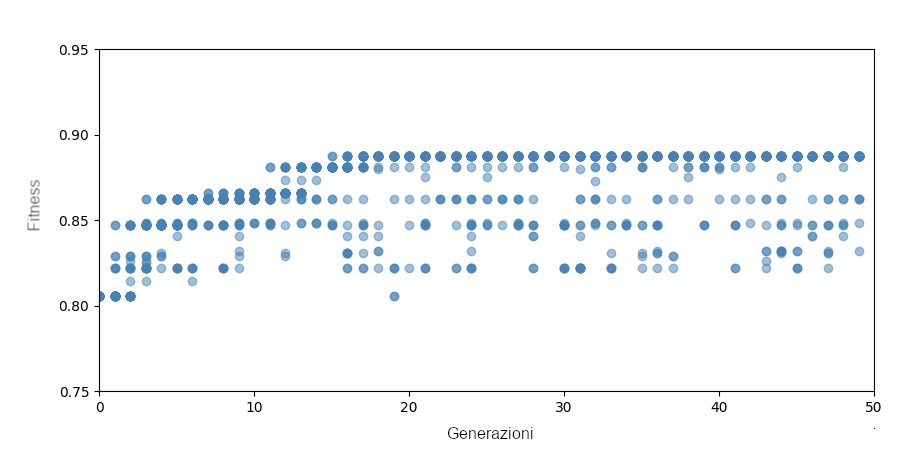
\includegraphics[width=1\columnwidth]{tesi/conf1} 
    \caption{Andamento valori di fitness di un instanza di prova testata con Conf1}
\end{figure}

Per cercare subito un confronto la prima modifica è stata nella \emph{mating\_pool\_size}, portandola a 40 (da 20) (Figura 5.5), questo ha aumentato notevolmente la diversificazione ed ha trovato soluzioni con un valore di fitness migliore delle soluzioni migliori con la Conf1. 

\begin{figure}[!ht] 
    \centering 
    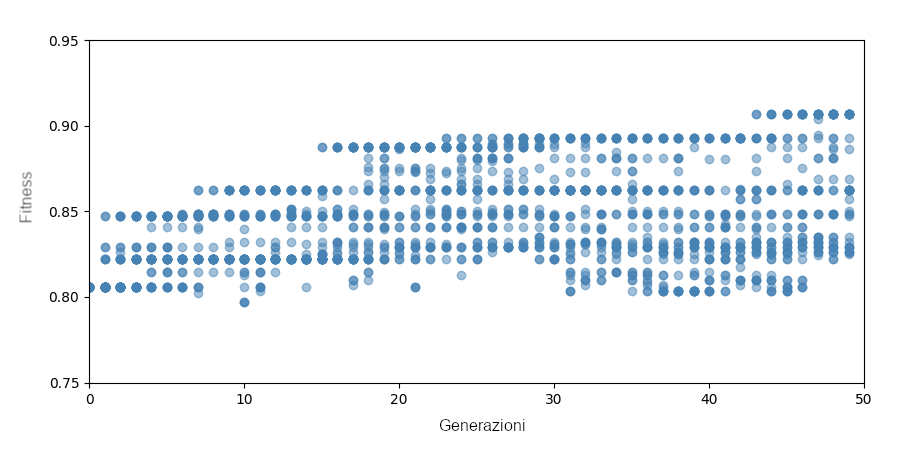
\includegraphics[width=1\columnwidth]{tesi/conf2} 
    \caption{Andamento valori di fitness di un instanza di prova testata con Conf2}
\end{figure}

Questo ha indicato come sicuramente sono presenti soluzioni migliori ottenibili con lo stesso numero di generazioni. Come si può notare, la Conf2 ha molta diversificazione, quindi l'obbiettivo di una nuova configurazione era migliorare l'intensificazione e cercare di diminuire la diversificazione senza perdere le nuove soluzioni che hanno ottenuto un valore di fitness migliore. Si è provato a diminuire la \emph{mating\_pool\_size} e aumentare la \emph{elite\_size} per aumentare l'intensificazione, ma è stato chiaro da subito che un 10\% di \emph{elite\_size} era già il massimo ottenibile senza ridurre drasticamente la diversificazione. Quindi si è provato ad aumentare \emph{crossover\_prob} ma con scarso successo. Sono state tentate anche configurazioni con diverse \emph{mutation\_prob} ma aumentandola si otteneva comunque abbondante diversificazione e diminuendola, anche di poco, calava troppo. 

\noindent L'equilibrio è stato trovato con la \textbf{Conf15}:
\begin{itemize}
	\item\textbf{population\_size}: 50;
	\item\textbf{crossover\_prob}: 0,7 (70\%);
	\item\textbf{mutation\_prob}: 0,3 (30\%);
	\item\textbf{mating\_pool\_size}: 30;
	\item\textbf{elite\_size}: 5.
\end{itemize}

(Figura 5.6), una \emph{mating\_pool\_size} corrispondente al 60\% della popolazione, ha generato un bilanciamento ottimale fra intensificazione, diversificazione e velocità di esecuzione. Infatti un altro problema della Conf2, era che una \emph{mating\_pool\_size} di 40 faceva svolgere una generazione in molto più tempo rispetto alla Conf1, quindi, essendo che i test di confronto con la soluzione aziendale, sarebbero stati svolti non con un criterio di arresto basato sulle generazione ma sul tempo, è stato necessario diminuire la \emph{mating\_pool\_size}.

\begin{figure}[!ht] 
    \centering 
    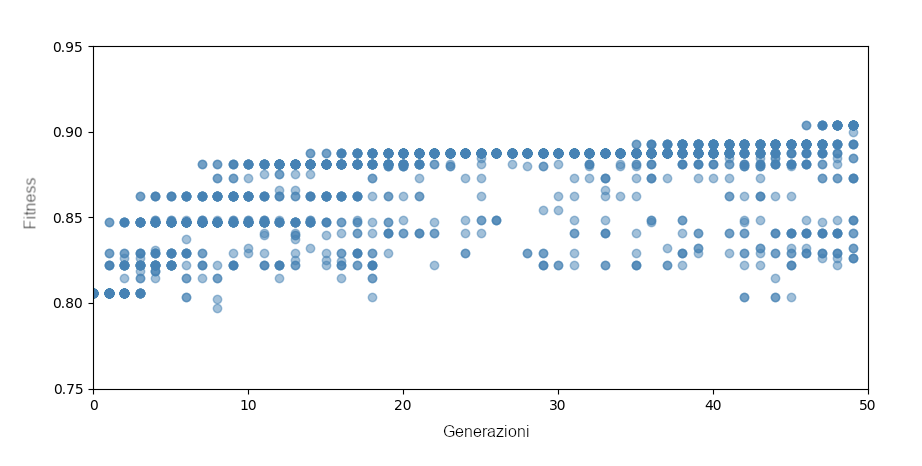
\includegraphics[width=1\columnwidth]{tesi/conf15} 
    \caption{Andamento valori di fitness di un instanza di prova testata con Conf15}
\end{figure}

\subsection{Analisi statistica}

50 istanze di prova diverse generate randomicamente, ciascusa istanza ha:
\begin{itemize}
	\item 1 solo tipo di foglio;
	\item 20 item obbligatori più 0 o 6 o 12 item opzionali;
	\item 0 o metà o tutti gli item obbligatori di una classe hanno margini;
	\item 0 o 20 precedenze, ovvero o nessun item obbligatorio ha precedenze oppure tutti gli obbligatori hanno una precedenza diversa.
\end{itemize}

Le seguenti medie sono ottenute sui valori di fitness della soluzione miglire, per ogni istanza, e il tempo (in secondi) impiegato per eseguire le 50 generazioni.

\noindent\textbf{Conf1}
\begin{itemize}
	\item\textbf{Fitness}: 0.7785907496795459
	\item\textbf{Tempo}: 26.64 
\end{itemize}
\textbf{Conf2}
\begin{itemize}
	\item\textbf{Fitness}: 0.7804101596824722
	\item\textbf{Tempo}: 27.76
\end{itemize}
\textbf{Conf15}
\begin{itemize}
	\item\textbf{Fitness}: 0.780764190701669
	\item\textbf{Tempo}: 27.26
\end{itemize}
Si può notare che da questi risultati si ottiene una configurazione migliore, tuttavia di tratta solo di risultati basati su determinate istanze. È importante sottolineare che tramite un t-test non sono stati rilevati sufficenti risultati per affermare che a livello statistico una configurazione è migliore di un altra. 

\section{Codifica}




pilot, perturbate, conf, chromosome, fitness (placement), retriveNestedSheet













% \intro{Breve introduzione al capitolo}\\

% \section{Tecnologie e strumenti}
% \label{sec:tecnologie-strumenti}

% Di seguito viene data una panoramica delle tecnologie e strumenti utilizzati.

% \subsection*{Tecnologia 1}
% Descrizione Tecnologia 1.

% \subsection*{Tecnologia 2}
% Descrizione Tecnologia 2

% \section{Ciclo di vita del software}
% \label{sec:ciclo-vita-software}

% \section{Progettazione}
% \label{sec:progettazione}

% \subsubsection{Namespace 1} %**************************
% Descrizione namespace 1.

% \begin{namespacedesc}
%     \classdesc{Classe 1}{Descrizione classe 1}
%     \classdesc{Classe 2}{Descrizione classe 2}
% \end{namespacedesc}


% \section{Design Pattern utilizzati}

% \section{Codifica}
